To get ready for solving general hydrodynamics problems 
in 1D, let us visit the simple advection problem. Consider 
a 1D domain in the coordinate x, ranging from $x=-L/2$ to 
$x=+L/2$ for some value of $L$. 
In this exercise we take $L=10$, but your program should 
keep this a free variable. Let us investigate the time 
evolution of a function $q(x, t)$ within this domain. We 
require $q(x, t)$ to obey the advection equation
\begin{equation}
    \pder{q(x,t)}{t}+v\cdot\pder{q(x,t)}{x}=0
\end{equation}
where $v>0$ is a constant. Let us take $v=1$. For this 
simple problem we know the analytic solution: 
\begin{equation}
    q(x, t>0) = q(x-vt, t=0),
\end{equation}
where we impose the periodic boundary condition implicitly. 
Let us new try to solve this equation numerically. We set 
up a grid in x with $N=100$ equally spaced grid points 
between $x=-L/2$ and $x=+L/2$ and with $\Delta x$ being the 
cell size. Furthermore, we add one ghost cell on each side 
to make the implementation of the boundary conditions 
easier.  In total we thus have 102 grid points in $x$. 
As initial condition we set
\begin{equation}
    q(x,0)=
    \begin{cases}
        1 &  \textnormal{for }x<0, \\
        0 &  \textnormal{for }x\geq0.
    \end{cases}
\end{equation}
As boundary condition we impose $q(-L/2, t)=1$ and 
$q(L/2,t)=0$, which is enforced simply by (re-)setting the 
values of $q$ in the ghost cells to the boundary value 
after each time step. Integrate in time from $t=0$ to 
$t=3$ using 100 equal-size time steps $\Delta t$.

\paragraph{1. Write a program to perform this numerical 
    integration using the symmetric numerical derivative 
    operator $(q_{i+1}-q{i-1})/(2\Delta x)$. Show that this 
    scheme will lead to a numerical instability.
} \ \\
    \\
    Code for $1D$ advection:
    \lstinputlisting[firstline=4, lastline=29]{../code/advection.py}
    \newpage\noindent
    Plotting:
    \lstinputlisting[firstline=6, lastline=35]{../code/task_1.py} \ \\
    As one can see in the plot below, the 
    symmetrical scheme leads to high-frequency 
    oscillations near $x=0$.
    \begin{figure}[h!]
        \centering
        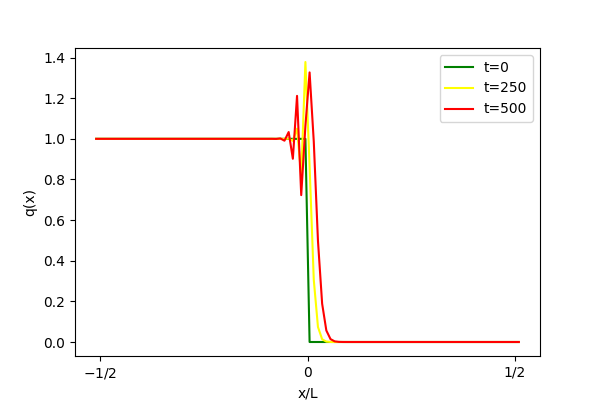
\includegraphics[width=.6\textwidth]{../figures/symmetric_1.png}
        \caption{Symmetrical numerical derivative leads to unstability.}
    \end{figure} \ \\ 

\newpage
\paragraph{2. Now use the one-sided numerical derivative 
    operator $(q_i-q_{i-1})/\Delta x$. Show that this 
    so-called upwind scheme stays stable.
} \ \\
    \begin{figure}[h!]
        \centering
        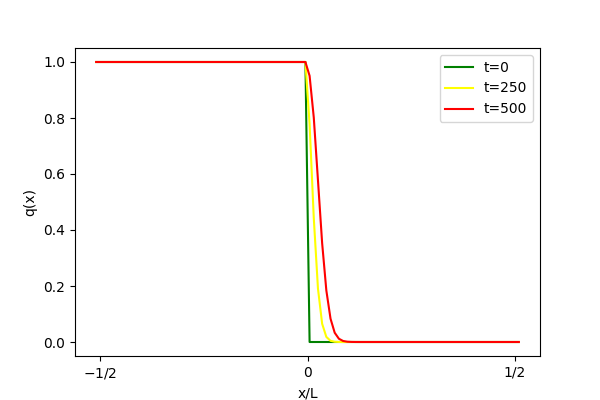
\includegraphics[width=.6\textwidth]{../figures/upwind_2.png}
        \caption{Upwind method leads to stable solution.}
    \end{figure} \ \\ 

\paragraph{3. Now use the one-sided numerical derivative 
    operator $(q_{i+1}-q_i)/\Delta x$. Show that this 
    approach is unstable again.
} \ \\
    \begin{figure}[h!]
        \centering
        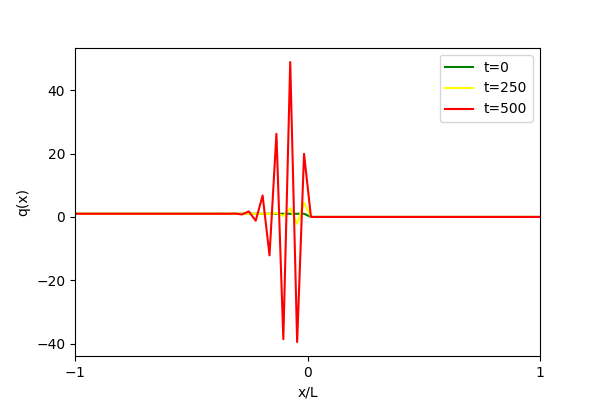
\includegraphics[width=.6\textwidth]{../figures/downwind_3.png}
        \caption{Downwind method leads to instability.}
    \end{figure} \ \\ 

\newpage \noindent
A good way to visualize the stability properties of the 
different numerical methods is to plot the values of 
$q(x,t)$ across the entire computational domain at 
different times. This exercise demonstrates that only the 
upwind advection algorithm leads to a stable solution. \\
\\
Let us investigate this scheme further, and from now on 
only use the upwind method.

\paragraph{4. Put the left boundary condition to 
    $q(-L/2,t)=0.5$. What happens, and why?
} \ \\
    % \lstinputlisting[firstline=38, lastline=38]{../code/task_1.py}
    \begin{figure}[h!]
        \centering
        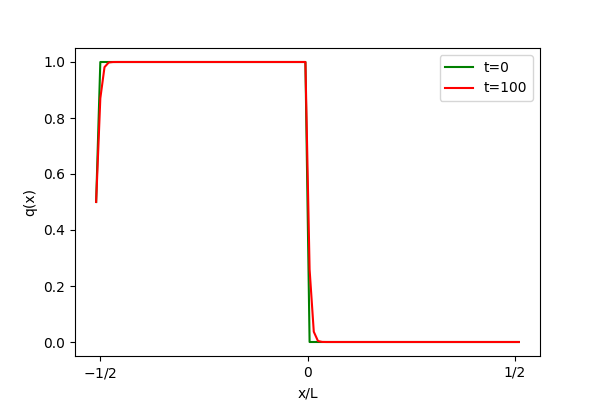
\includegraphics[width=.6\textwidth]{../figures/upwind_4.png}
        % \caption{}
    \end{figure} \ \\ 
    Near the left edge, the expected behavior can 
    be seen. Apart from that, the overall structure 
    of the curve is the same as for the initial 
    boundary condition. 

\paragraph{5. Reset, and put the right boundary condition 
    to $q(+L/2,t)=0.5$. What happens, and why?
} \ \\ 
    % \lstinputlisting[firstline=39, lastline=39]{../code/task_1.py}
    \begin{figure}[h!]
        \centering
        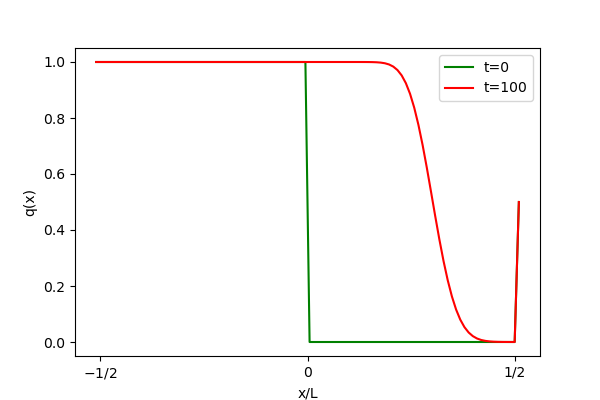
\includegraphics[width=.6\textwidth]{../figures/upwind_5.png}
        % \caption{}
    \end{figure} \ \\ 
    Contrary to the last plot, the expected smooth 
    rise towards the boundary condition can not 
    be seen here.
    This is because we're using the upwind method, 
    where information is transported only from left
    to right.

\paragraph{6. Reset again, and use a $10\times$ smaller 
    time step, i.e. take 1000 time steps between $t=0$ and 
    $t=3$. What is the difference in the result at $t=3$? 
    Does it become better or worse?
} \ \\
    \begin{figure}[h!]
        \centering
        \begin{minipage}{.5\linewidth}
          \centering
          \subfloat[100 time steps]{
            \label{:a}
            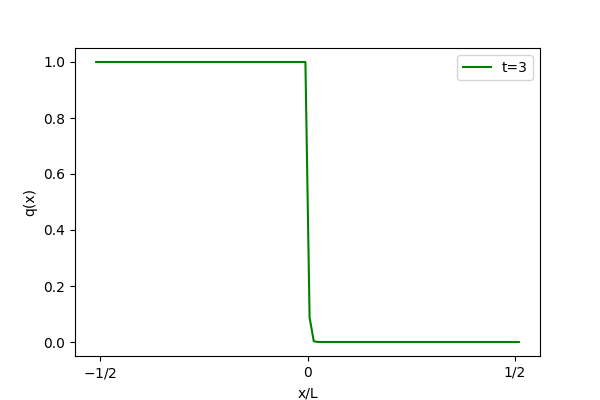
\includegraphics[scale=.6]{../figures/upwind_6_0.png}
          }
        \end{minipage}%
        \begin{minipage}{.5\linewidth}
          \centering
          \subfloat[1000 time steps]{
            \label{:b}
            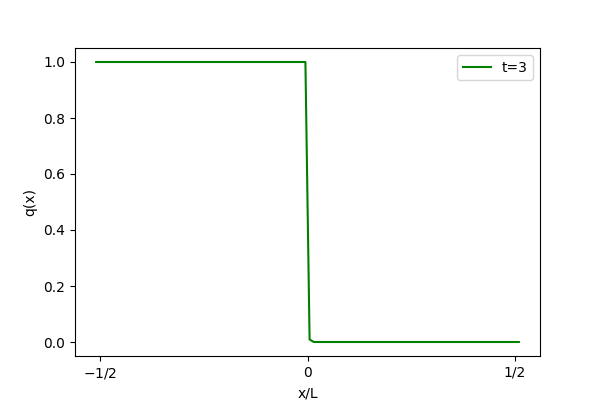
\includegraphics[scale=.6]{../figures/upwind_6.png}
          }
        \end{minipage}
        % \caption{}
    \end{figure} \ \\
    The behavior at $x=0$ is smoother when using 
    smaller time steps. It becomes better.

\paragraph{7. Repeat, but now use a $10\times$ larger time 
    step, i.e. take 10 time steps between $t=0$ and $t=3$. 
    Explain what happens.
} \ \\
    \begin{figure}[h!]
        \centering
        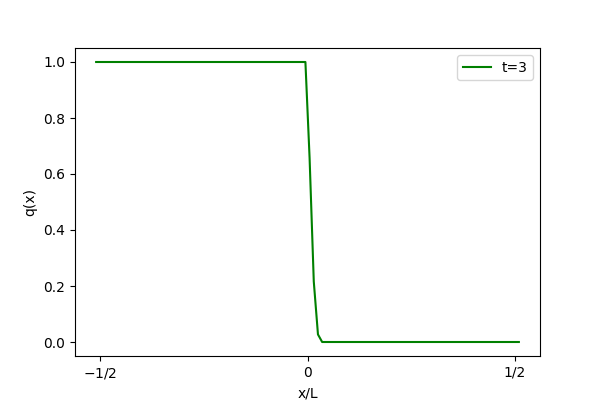
\includegraphics[width=.6\textwidth]{../figures/upwind_7.png}
        \caption{10 time steps}
    \end{figure} \ \\ 
    Less time steps lead to a less steep descent 
    from 1 down to 0.

